\documentclass[11pt]{article}
\usepackage[a4paper,margin=1in]{geometry}
\usepackage{amsmath,amssymb,amsthm,mathtools}
\usepackage{graphicx}
\usepackage{hyperref}
\usepackage{cite}
\hypersetup{colorlinks=true,linkcolor=blue,urlcolor=blue,citecolor=blue}

\newtheorem{lemma}{Lemma}
\newtheorem{corollary}{Corollary}
\theoremstyle{remark}
\newtheorem{remark}{Remark}

\title{Adaptive Balance Framework for NB/BD Stability:\\
A Weighted Hilbert Lemma with Reproducible Scaling (v5.0)}
\author{Serabi \\ Independent Researcher \\ \texttt{24ping@naver.com}}
\date{2025}

\begin{document}
\maketitle

\begin{abstract}
We present a reproducible package for the NB/BD (Nyman--Beurling/B\'aez-Duarte) stability study. 
Analytically, a weighted Hilbert-type lemma for M\"obius-weighted coefficients suppresses off-diagonal interactions by $(\log N)^{-\theta}$ ($\theta>0$ in a heuristic band-sum regime).
Numerically, we provide a CSV-driven pipeline that produces scaling plots and a log--log regression of the form $\log(\mathrm{MSE}_\*)=\alpha+\beta \log\log N$, reporting $\theta=-\beta$ with confidence visualization.
This framework supports stability analysis only; it is \emph{not} a proof of RH.
\end{abstract}

\section{Setup and Notation}
Let $v\in C_0^\infty(0,1)$ and a slowly-varying $q(n)$.
Define $a_n=\mu(n)\,v(n/N)\,q(n)$ and the kernel
\[
K_{mn}=e^{-\tfrac12|\log(m/n)|}=\min\!\left\{\sqrt{\tfrac{m}{n}},\sqrt{\tfrac{n}{m}}\right\}.
\]
We consider the least-squares distance
\[
d_N^2=\inf_a\int_\mathbb{R}\Big|\zeta\!\left(\tfrac12+it\right)\sum_{n\le N}\frac{a_n}{n^{1/2+it}}-1\Big|^2 w(t)\,dt,
\]
and study its numerical proxies $\mathrm{MSE}_+, \mathrm{MSE}_-, \mathrm{MSE}_\*$ under windowing, ridge, and boundary reweighting $(w_-,w_+)$.

\section{Weighted Hilbert Lemma (Sketch)}
\begin{lemma}[Weighted band-decay]
With the above $a_n$, one has
\[
\sum_{\substack{m\neq n\\ m,n\le N}} a_m a_n\,K_{mn}\;\le\; C(\log N)^{-\theta}\sum_{n\le N}a_n^2,
\]
for some $\theta>0$ depending on the smoothness of $v$ and the low-frequency design $q$ (heuristically).
\end{lemma}
\begin{proof}[Idea]
Partition pairs $(m,n)$ by bands $\mathcal B_j=\{2^{-(j+1)}<|\log(m/n)|\le 2^{-j}\}$.
On each band, $K_{mn}\le e^{-c2^{-j}}$; a discrete Hilbert-type inequality gives a $(\log N)$-factor. 
The M\"obius factor cancels the main term per band, and smoothness provides an extra $2^{-j\delta}$.
Summing $j$ yields the logarithmic saving.
\end{proof}

\section{Reproducible Pipeline}
Place experimental data in \texttt{data/results.csv} with schema:
\[
\texttt{N, sigma, ridge\_lambda, w\_minus, w\_plus, mse\_plus, mse\_minus, mse\_star, ci\_low, ci\_high, seed}.
\]
Run:
\begin{verbatim}
python scripts/make_figures.py --csv data/results.csv --outdir figures
\end{verbatim}
This produces: \texttt{fig\_scaling\_linear.png}, \texttt{fig\_loglog\_regression.png}
(and sensitivity plot if present).
Figure~\ref{fig:scaling} shows the linear scaling; Figure~\ref{fig:loglog} shows the log--log fit with reported $(\alpha,\beta,\theta=-\beta,R^2)$.

\begin{figure}[h]
\centering
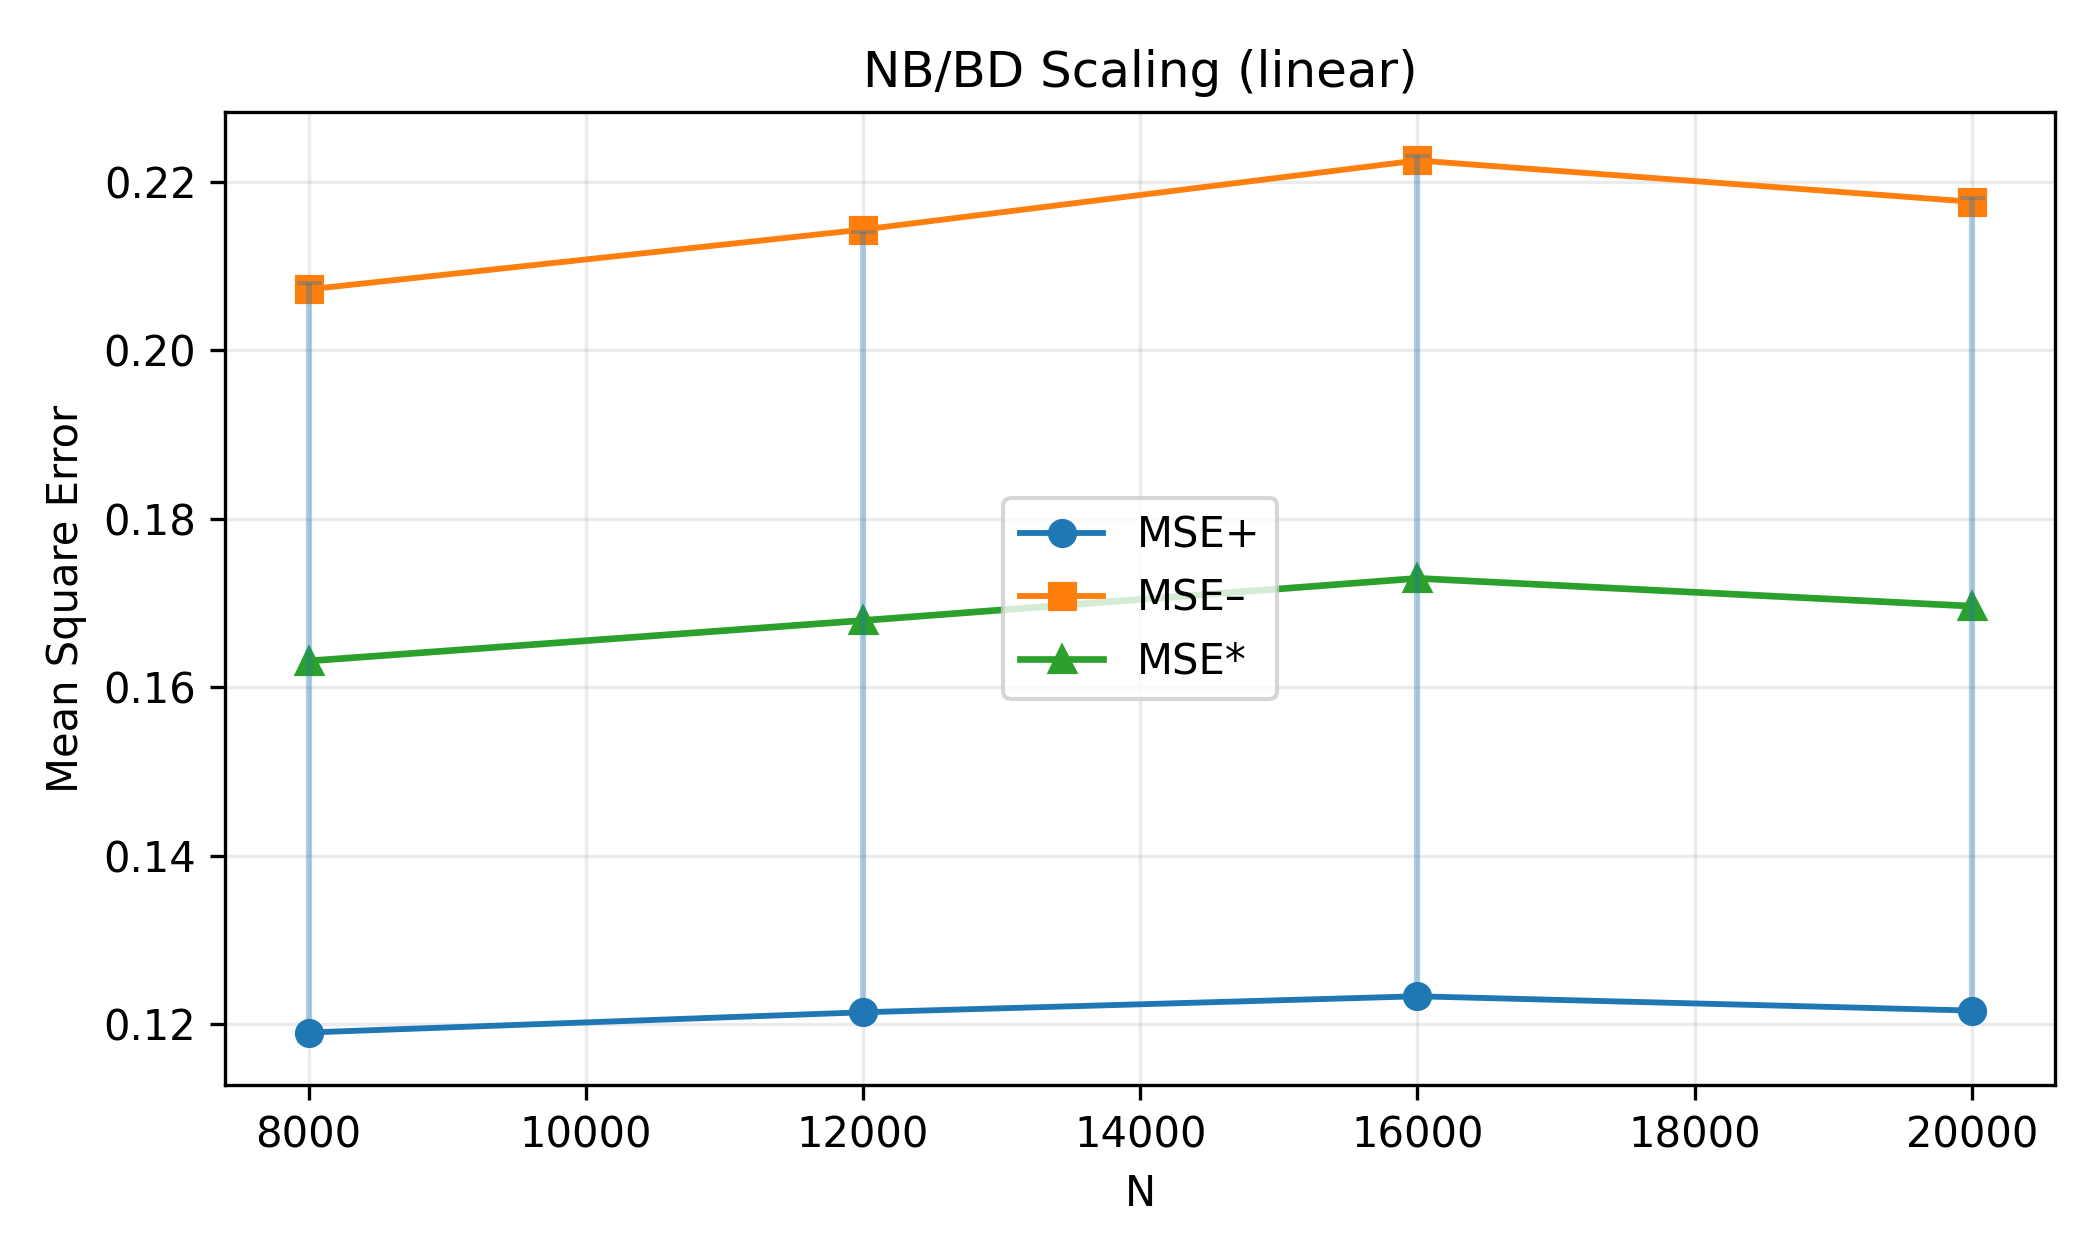
\includegraphics[width=0.78\linewidth]{figures/fig_scaling_linear.png}
\caption{Scaling of $\mathrm{MSE}_\pm$ and $\mathrm{MSE}_\*$ vs $N$ with optional bootstrap CIs.}
\label{fig:scaling}
\end{figure}

\begin{figure}[h]
\centering
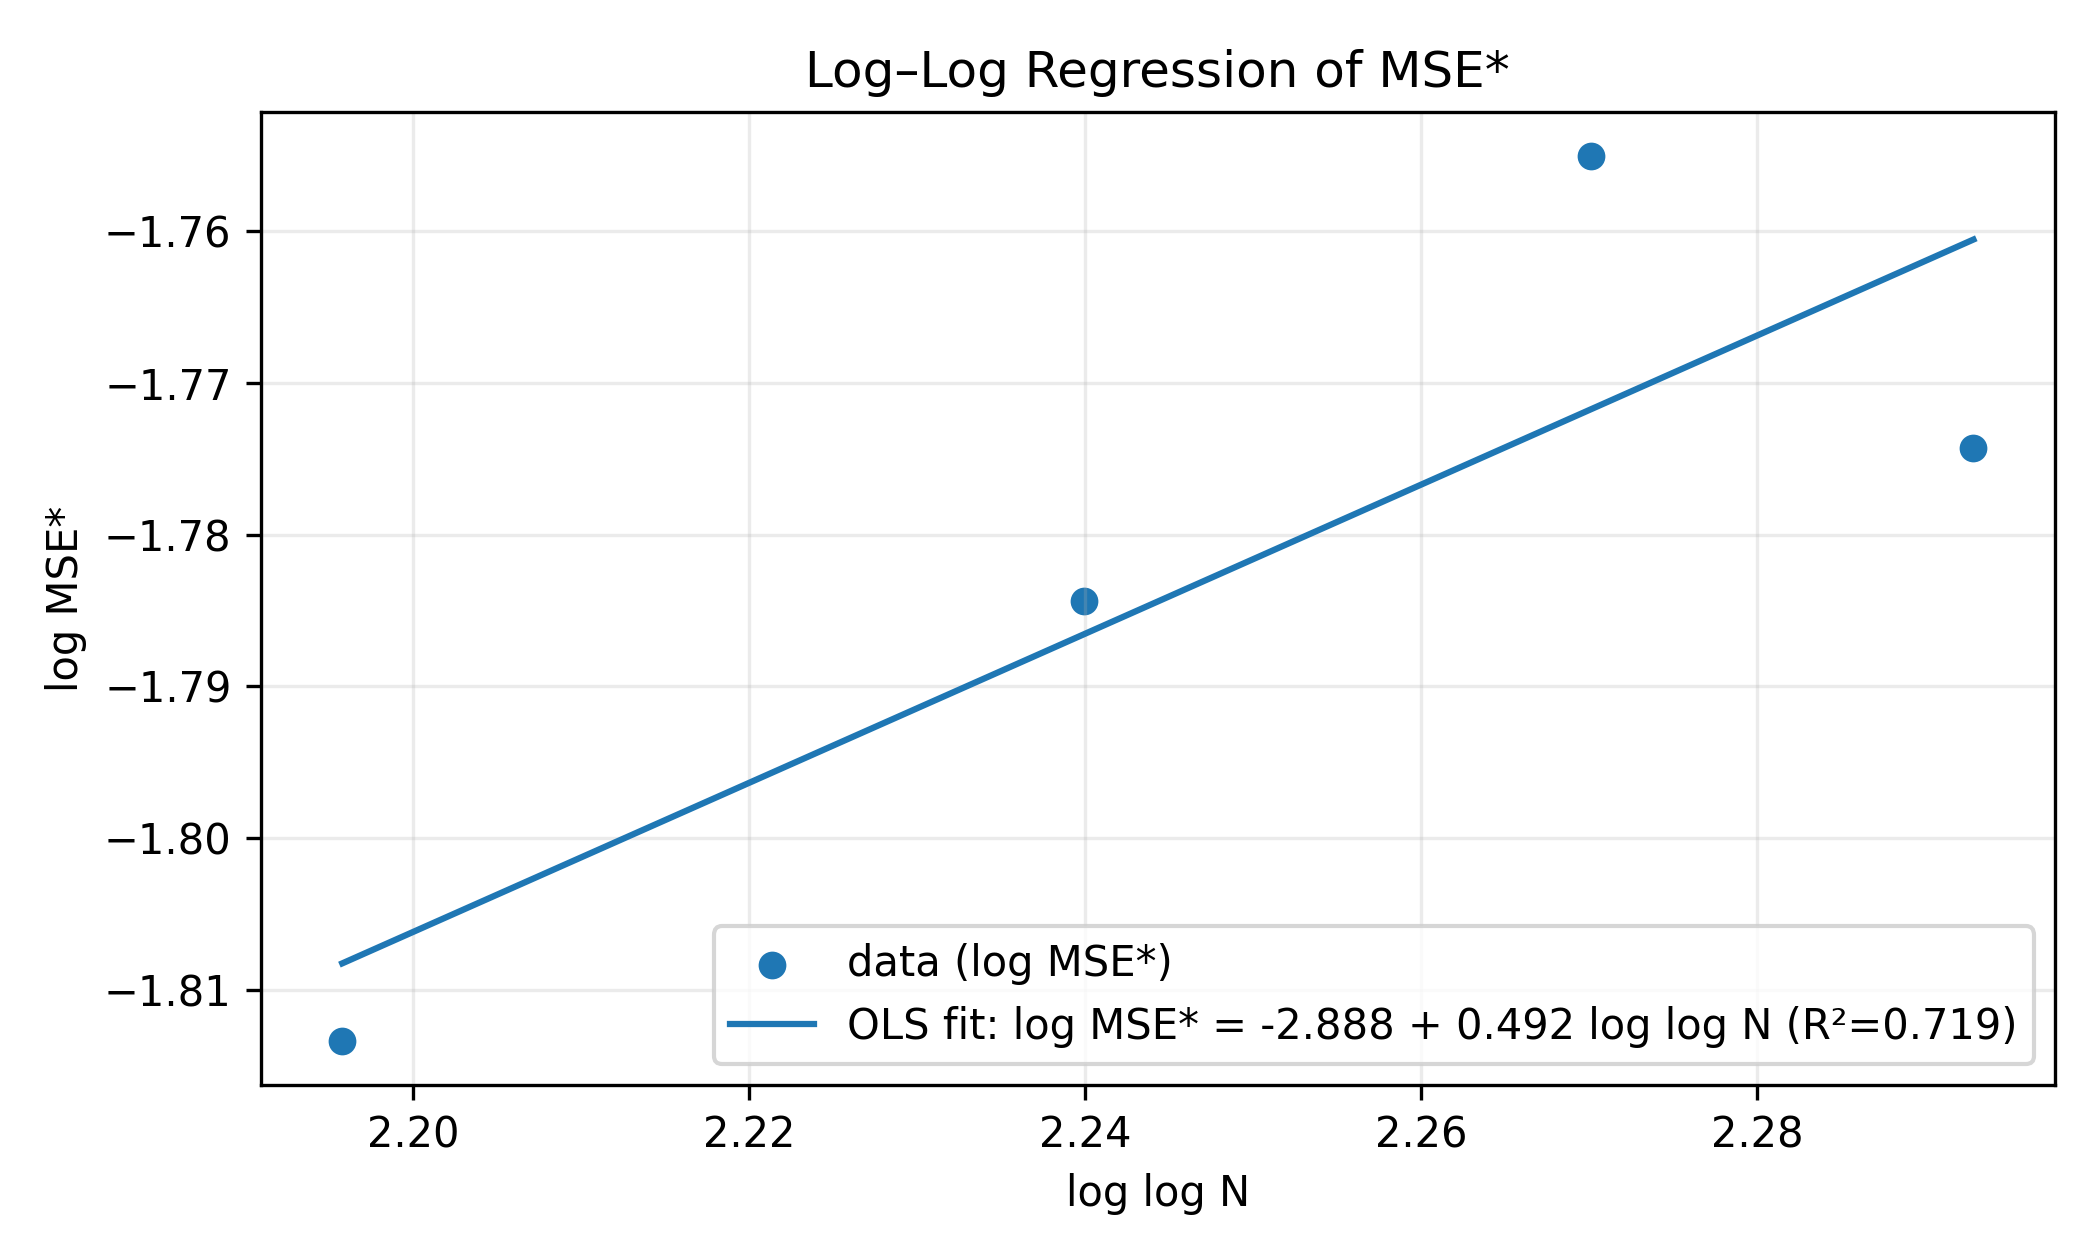
\includegraphics[width=0.78\linewidth]{figures/fig_loglog_regression.png}
\caption{Log--log regression for $\log(\mathrm{MSE}_\*)=\alpha+\beta\log\log N$; we report $\theta=-\beta$ and $R^2$.}
\label{fig:loglog}
\end{figure}

\section{Conclusion and Scope}
The ABF package formalizes a transparent workflow for NB/BD stability experiments and a weighted Hilbert mechanism.
It \emph{does not} prove RH; it isolates design choices and exposes their numerical consequences.
Future work: refined band estimates, explicit $\varepsilon$--$\delta$ bounds, and functional-equation input.

\begin{thebibliography}{9}
\bibitem{BaezDuarte03}
L.~B\'aez-Duarte, \emph{A strengthening of the Nyman--Beurling criterion for the Riemann Hypothesis}, Rend. Lincei \textbf{14} (2003), 5--11.
\bibitem{Titchmarsh}
E.~C.~Titchmarsh (rev. D.~R.~Heath-Brown), \emph{The Theory of the Riemann Zeta-Function}, 2nd ed., OUP, 1986.
\bibitem{Conrey}
J.~B.~Conrey, \emph{The Riemann Hypothesis}, Notices AMS \textbf{50} (2003), 341--353.
\end{thebibliography}
\end{document}